%\documentclass[11pt,a4paper,oldfontcommands]{memoir}
\documentclass[oneside,11pt,a4paper,oldfontcommands]{book}
\usepackage[utf8]{inputenc}
\usepackage[T1]{fontenc}
\usepackage{microtype}
\usepackage[dvips]{graphicx}
\usepackage{times}
\usepackage{titlesec}
\usepackage{wrapfig}
\usepackage{float}
\usepackage{xcolor}
\usepackage{setspace}




\usepackage[
breaklinks=true,colorlinks=true,
%linkcolor=blue,urlcolor=blue,citecolor=blue,% PDF VIEW
linkcolor=black,urlcolor=black,citecolor=black,% PRINT
bookmarks=true,bookmarksopenlevel=2]{hyperref}

\usepackage{geometry}
% PDF VIEW
% \geometry{total={210mm,297mm},
% left=25mm,right=25mm,%
% bindingoffset=0mm, top=25mm,bottom=25mm}
% PRINT
%\geometry{total={210mm,297mm},
%left=20mm,right=20mm,
%bindingoffset=10mm, top=25mm,bottom=25mm}

\onehalfspacing
%\linespread{1.3}

%%% CHAPTER'S STYLE
%\chapterstyle{ger}
%\chapterstyle{madsen}
%\chapterstyle{ell}
\titleformat{\chapter}
  {\Large\bfseries} % format
  {}                % label
  {0pt}             % sep
  {\huge}  
%%% STYLE OF SECTIONS, SUBSECTIONS, AND SUBSUBSECTIONS
%\setsecheadstyle{\Large\bfseries\sffamily\raggedright}
%\setsubsecheadstyle{\large\bfseries\sffamily\raggedright}
%\setsubsubsecheadstyle{\bfseries\sffamily\raggedright}


%%% STYLE OF PAGES NUMBERING
%\pagestyle{companion}\nouppercaseheads 
%\pagestyle{headings}
%\pagestyle{Ruled}
\pagestyle{plain}
%\makepagestyle{plain}
%\makeevenfoot{plain}{}{\thepage}{}
%\makeoddfoot{plain}{}{\thepage}{}
%\makeevenhead{plain}{}{}{}
%\makeoddhead{plain}{}{}{}

\def\code#1{\texttt{#1}}


%\maxsecnumdepth{subsection} % chapters, sections, and subsections are numbered
%\maxtocdepth{subsection} % chapters, sections, and subsections are in the Table of Contents


%%%---%%%---%%%---%%%---%%%---%%%---%%%---%%%---%%%---%%%---%%%---%%%---%%%

\begin{document}

%%%---%%%---%%%---%%%---%%%---%%%---%%%---%%%---%%%---%%%---%%%---%%%---%%%
%   TITLEPAGE
%
%   due to variety of titlepage schemes it is probably better to make titlepage manually
%
%%%---%%%---%%%---%%%---%%%---%%%---%%%---%%%---%%%---%%%---%%%---%%%---%%%
\thispagestyle{empty}

{%%%
\sffamily
\centering
\Large
~\vspace{\fill}

{\huge 
An Open-Source Event-Based SCADA System for the Power Grid
}

\vspace{2.5cm}

{\LARGE
Trevor Aron
}

\vspace{3.5cm}

A project report submitted to the Johns Hopkins University in
conformity with the requirements for the degree of Master 
of Science in Engineering\\ 

\vspace{3.5cm}

Advisors: Dr. Yair Amir, Thomas Tantillo

\vspace{\fill}

May 2017

%%%
}%%%

%%%---%%%---%%%---%%%---%%%---%%%---%%%---%%%---%%%---%%%---%%%---%%%---%%%
%%%---%%%---%%%---%%%---%%%---%%%---%%%---%%%---%%%---%%%---%%%---%%%---%%%

\chapter*{Acknowledgements}

\indent \indent I would like to thank Marco Platania. Marco Platania really introduced me to
what SCADA actually is. We came up with the scenario that I would end up building
together after scouring the internet for youtube videos of HMI demos. Marco
was also the first person to realize the limitations of pvbrowser and split
the HMI and Data Acquisition portions, leading to the creation of the new SCADA 
architecture I am now presenting. \\

\indent I would like to thank Tom Tantillo for his contributions and 
his constant support.  He worked
with me tirelessly to get this made. Tom has an amazing ability to get things
done, and done well, no matter how impossible it seems.
He has served as one of my main mentors, helping me with everything from 
writing posters to drafting emails. I am appreciative for the time
we have been able to chat in the DSN lab. \\

\indent I must also thank Yair Amir. He was my professor in Intermediate Programming, 
Distributed Systems, and Advanced Distributed System. It was he who made me
interested in systems. It was also he who had the vision for intrusion-tolerant
SCADA and fortunately invited me to help. I truly admire his desire to
protect the nations infrastructure for the good of society. \\

\indent 
Finally I would like to thank Amy Babay. Amy Babay has helped me in countless ways
and is always there to answer my questions or clue me in as to what is happening. 
She has made significant contributions and helped me edit this report .\\

\indent
This work was supported in part through a Pistritto Fellowship Grant. \\
\clearpage
\tableofcontents*

\clearpage

%%%---%%%---%%%---%%%---%%%---%%%---%%%---%%%---%%%---%%%---%%%---%%%---%%%
%%%---%%%---%%%---%%%---%%%---%%%---%%%---%%%---%%%---%%%---%%%---%%%---%%%
\chapter{Abstract}

\indent \indent
We present the design and construction of an open-source event-based SCADA system. There are four main motivations 
for this work: making it easier to replicate the SCADA Master, making the
system more scalable, increasing security, and facilitating adoption
 through open-source. A key component of our architecture
is the use of a PLC/RTU proxy that facilitates scalability and increases
the security, while maintaining backward compatibility with existing
SCADA equipment. Our system architecture and software components are used
as part 
of the Spire intrusion-tolerant SCADA system for the power grid \cite{Spire}. \\


\chapter{Introduction}

%The key component of this architecture is the RTU/PLC Proxy.
%This additional machine allows the SCADA system to be fully backwards compatible with devices while
%making sure that updates from devices are delivered to the core system as changes occur. Additionally
%this extra component provides an additional layer of security to the SCADA system.

%\indent \indent
%SCADA systems monitor and control much of the world's critical infrastructure. Recently, they
%have been under attack by malicious actors. To increase SCADA Security, some researchers have
%been working towards building byzantine fault tolerant replicated SCADA systems. However,
%current SCADA architectures are are unfit for replication. \\

%\indent This document presents the construction of an open-source event-based SCADA 
%architecture.
%The aim of this work is to build a SCADA system that lends it self for replication,
%is scalable, and is still backwards compatible with current SCADA equipment. 
%Additionally, this new architecture has the added benefit of providing device security. \\

% scalable, and has an 
%easy to work with architecture that is still backwards compatible with
%SCADA equipment. The key component of this architecture is the RTU/PLC Proxy. This additional 
%component is used to build a SCADA system architecture that is scalable, incorporates
%device security, easy to replicate, and backwards compatible with existing SCADA 
%equipment in the field.\\


\indent \indent SCADA stands for Supervisory Control and Data Acquisition. 
SCADA systems are used 
to monitor and control physical devices in critical infrastructure applications.
Such applications include railways, electrical grids, power generation,
waste management, water supply, and factories ~\cite{CyberWarfare}. \\

\begin{figure}[ht]
  \begin{center}
  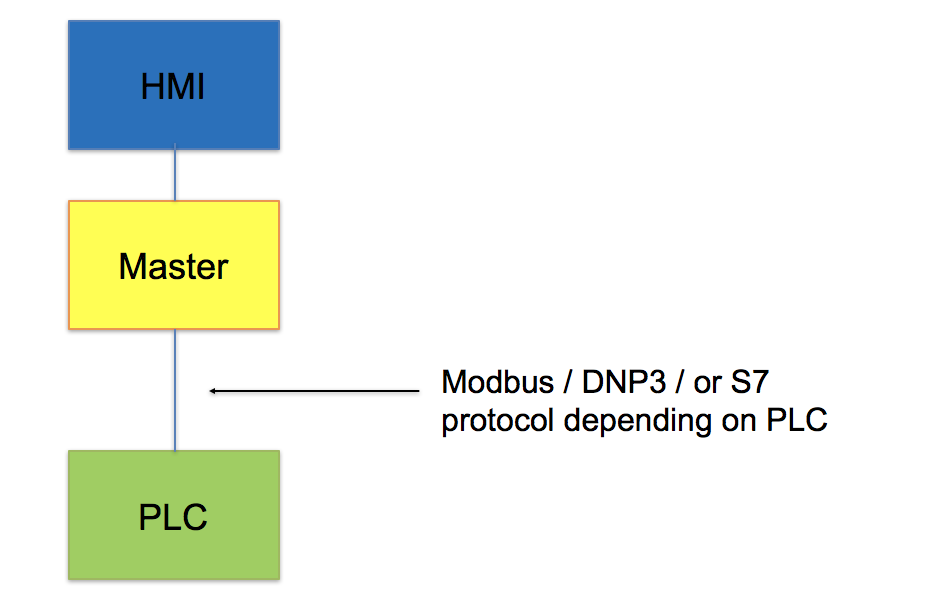
\includegraphics{normal_scada}
  \caption{Architecture of a SCADA System}
  \label{fig:1}
  \end{center}
\end{figure}

\indent
SCADA systems vary depending on the specific application being monitored and controlled.
These differences can influence the topology of the network and the
protocols being used to communicate between the Master and PLC \cite{SCADANetworks}.
SCADA devices and equipment are also
mainly vendor locked, which means the specific protocols and components
change from system to system. However,
SCADA systems generally share the basic architecture described in Figure \ref{fig:1}. 
This shows the three main portions of any SCADA system: the Human Machine
Interface (HMI), the SCADA Master, and the Programmable Logic Controller (PLC) or Remote 
Terminal Unit (RTU). \\

\indent
The Human Machine Interface is a program that visualizes the data to a Human operator
and allows said operator to issue commands that make changes to the system. 
The visual display of an HMI are specific to the critical infrastructure
system or scenario being monitored and controlled. Each HMI typically presents
a user interface that visually shows a representation of the physical equipment.
For example, an HMI monitoring water levels may have an image of a tank with
a variable amount of water in it. An HMI monitoring a power grid may have 
dials with voltage outputs and buttons that correspond to switches. \\

\indent
Programmable Logic Controllers and Remote Terminal Units are the devices that
communicate directly with the physical equipment in the field that need to be
monitored and controlled. RTUs are a little more intelligent
than PLCs and are usually outfitted with alternative communication systems such as radio.
They may also perform some small automated control tasks. They are specifically used by 
industrial control systems. PLCs are a bit more generic, and most hobbyist boards (such as Arduino's)
can be considered as a PLC. RTUs and PLCs in SCADA systems are usually vendor 
created, closed-source devices. They also communicate with legacy communication protocols, 
which have been around since the 1970s and 1980s. 
The American Gas Association's AGA-12 standard states that there are between 150-200
different SCADA communication protocols \cite{SCADANetworks}. Some popular
protocols include Modbus, DNP3, and Siemens S7. \\

\indent
The SCADA Master is the brain of the system. All monitoring and state messages 
from the PLCs are collected by the SCADA Master, giving it a global
view of the state of the system. All commands from the HMI first go to the
SCADA Master for processing before they are sent to a PLC. 
The SCADA Master communicates with the PLCs and RTUs using the SCADA communication 
protocol that each RTU or PLC supports. The SCADA Master typically
has automated control and alerting capabilities. They also contain a historian which
keeps an audit trail of operational data \cite{CyberWarfare}.  \\

\indent 
SCADA systems were designed in the earlier days of computing before cyber security was
a real consideration. Traditionally, they have relied on two main factors for security:
obscurity and private networks. Since most SCADA devices are proprietary, there
is little information of how they operate available to the public. Additionally, many
SCADA systems where designed to operate on private networks. However, this
is not a real solution: air gaps can be breached, and obscurity is
not a good form of security when the attackers are nation states. Additionally,
the air gaps are going away as using IP Networks is cheaper and easier. \\

Stuxnet is a virus, first identified in 2010, that was discovered to
target Siemens SCADA systems. Specifically, it was aimed at the
Siemens SCADA systems that controlled nuclear enrichment facilities in Iran.
The system it attacked was air gapped, but the virus entered via a USB
stick and then spread by copying itself on
remote drives and attacking other computers on the same local area network through
a zero day vulnerability. It infected computers that
were used to modify and program PLCs and used this to insert malicious code
into a PLC that would make it function incorrectly \cite{Stuxnet}. \\

With the onset of Stuxnet, SCADA system security became prominent. The test in \cite{WhosAttacking} shows
the extent of the threat. They set up a honey pot of PLCs connected to the internet.
In a month time frame there where over 39 attacks from 14 different countries. 
Many PLCs and RTUs are configured incorrectly or connected to the
internet such that employees can access and modify them from home. One can
find PLCs on the internet with a basic search. The website Shodan is a 
search engine designed to discover Internet of Things (IOT) devices on the internet.
They have an entire section devoted to finding industrial control equipment by looking for
IP connected devices with common SCADA protocol ports open, which helps
illustrate how poor current SCADA security is \cite{Shodan}. \\

\indent 
There are four main motivations for building this open-source
event-based system. The first is facilitating replication of the SCADA Master:
 because current SCADA Masters are very complex and use polling based protocols,
 they do not lend themselves to replication.
The second is scalability: an event-based system pushes less
data over the network.
The third is security: the PLC/RTU Proxy component in the event-based SCADA architecture
provides a powerful layer of security that existing RTUs and PLCs lack. 
The final motivation is facilitating adoption of this system through open-source. Below
we describe each motivation.\\

\section{Facilitating SCADA Master Replication}

\indent \indent
Replicating the SCADA Master opens the door for making SCADA systems more available:
a system could be replicated to be fault tolerant,
or, by using a byzantine fault tolerant algorithm, replicated to make the system intrusion tolerant -
allowing it to work even if components have been compromised by an intruder.
Specifically, this system was used to make Spire, an intrusion tolerant SCADA
system \cite{Spire}. \\

\indent 
In \cite{SurvivableSCADA}, Kirsch et al. built an intrusion-tolerant prototype 
based on a Siemens SCADA product for the power grid. They note that 
intrusion tolerant replication systems, such as Prime \cite{Prime}, assume that updates are 
client driven (event-based), while most SCADA systems process requests that are
server driven (polling). This mismatch caused them to create the intrusion tolerant timeout
protocol. This protocol is used to synchronize the SCADA Masters so that they poll the devices at the
same logical time. Not only is this protocol challenging to implement, it also negatively
impacts the system by increasing overhead. \\

\indent
By making an event-based system, the intrusion tolerant timeout protocol is no
longer needed, as masters no longer need to coordinate their polling with
each other. This makes replication
of the system much simpler and considerably decreases overhead.\\

\section{SCADA Scalability}

\indent \indent
There are two different SCADA protocol architectures. The first is a polling model, and
the second is an event-based model. An event-based model consists of the device only
sending updates to the master whenever there is a change of state. DNP3 is an
event-based protocol. The polling
model consists of the master sending requests for updates to the devices
at different polling intervals. Modbus is a polling protocol.\\

\indent
One of the issues with the polling model is that it does not scale. Each device
takes a constant amount of bandwidth. This is expensive. Some devices may transmit
a lot of data on each polling interval. There are some SCADA systems, like smart
grids, that are very large. There is an estimated 150,000,000 meters installed in Europe
\cite{EventMeters}. If the devices only
speak a protocol like Modbus, then there would be a massive amount of bandwidth
used. In addition the historian would have to store much more data. Event-based
models are more efficient because messages are sent only when the device state
has changed.\\

\indent
The need for SCADA scalability has been recognized by others in the field.
SAP and Schneider Electric have laid out their vision for the future of SCADA in \cite{nextgen}. 
They address that it is impossible to perform polling in large-scale SCADA systems, and
suggest the transition to event-driven architectures in the future. However, they stress
that future SCADA systems must stay backward compatible to work with existing devices.
The authors of \cite{EventMeters} were running
a smart grid monitoring system. In order to scale this monitoring, they created a new 
protocol and communication pattern. The drawback with this approach
is that it breaks backward compatibility. \\

\indent
The solution we propose includes a device, the PLC/RTU proxy, ideally colocated with  RTU and PLC devices. The RTU
proxy speaks multiple SCADA protocols (currently Modbus and DNP3, but it can be extended
to other protocols) and translates
this information to a generic IP format the SCADA master understands. The Proxy
can be designed such that it only pushes information when there is a change in state.
This solution makes all SCADA systems have more homogenous communication patterns despite
the devices that may need to be used.


\section{SCADA Security Concerns}

\indent \indent 
One of the weakest parts of a SCADA system are the devices. They are difficult to harden:
PLCs may have very limited computational abilities. They also often run on
real-time operating systems which are lighter weight, but provide less security. Thus, many
PLCs cannot support running a firewall \cite{SCADANetworks}. In
addition, because they run on real time operating systems, PLCs are more susceptible
to disruption from denial of service attacks. \\

\indent
Beyond the PLC itself, SCADA communication protocols are not secure. 
Most protocols typically do not support cryptographic primitives.
This is also due to the limited computing power of the devices. As a result, 
communication between the SCADA Master and device is unencrypted and most
 commands are unauthenticated. For
instance, Modbus messages are 
sent over the wire completely unencrypted, with no integrity checks,
and no authentication. If an adversary is on the same network as a 
device that speaks Modbus,
the adversary can send the PLC arbitrary commands and alter contents of
messages that the PLC and Master exchange \cite{SecureModbus}. In addition, because the
world of SCADA is vendor locked, many of these protocols have been
programmed from scratch for a particular device. Many of these implementations
are not robust and have bugs. In our own experiments with the ASE Test Set 2000
RTU emulation device, we found that it had bugs in it's implementation of DNP3. These
bugs are often an entry way for intruders. \\

There have been many efforts to harden PLCs. For instance,  the efforts in 
Fovino et al. propose a new Modbus protocol that is translated
by a middle gateway device into regular Modbus for backwards compatibility 
with devices \cite{SecureModbus}. However, this breaks backwards compatibility
 with masters. A broader approach has also been to attach  machines at
both ends, one at the SCADA Master, and the other at the RTU or PLC
\cite{SCADANetworks}. This acts as a bump in the wire
in which data is encrypted. To solve the firewall issue, there
has also been efforts to place small firewalls in front of each PLC in a network
\cite{SCADANetworks}. \\

The solution that we propose, the RTU/PLC proxy, solves these issues. The RTU Proxy is a 
machine that is placed in front of RTUs or PLCs on the network. It
translates commands from the Master into the specific PLC or RTU communication 
protocol for the corresponding device. This proxy runs a firewall for the devices
that it speaks to, removing them from direct access from the wide area network. Since
the proxy is a modern machine, and not a device board, it can also preform cryptographic
primitives. Thus, the information it gets from the SCADA Master has authentication, 
integrity, and confidentiality. It currently can speak DNP3 and Modbus, the two most
popular protocols used for power distribution SCADA systems, but can easily be
extended to speak any SCADA protocols, allowing the system to remain compatible with
any device.\\

\section{Adoption}

\indent \indent
Finally, the motivation to build this system entirely with open-source components is
to encourage usage and adoption in the SCADA community and help foster
an open source SCADA ecosystem. The efforts of Kirsch et al. in
\cite{SurvivableSCADA} are unfortunately unavailable
as Siemens decided not to release this product. By building an open-source
SCADA system, this work can be used as a base for SCADA security research.
The Spire system is able to leverage our work thanks to all of the components
being released as open-source.\\

\indent 
In addition, using open-source components enables the system to benefit as
different parts are improved with future research. OpenDNP3 \cite{OpenDNP3}
is currently maintained by a group that performs vulnerability research on SCADA
protocols. We use this for our DNP3 implementation, and the security of our
system will be improved from their work. We use OpenPLC \cite{OpenPLC} to emulate PLCs 
in this system. This integration benefits our system as OpenPLC is being designed to
be used as a vehicle for PLC security research, and when the security of OpenPLC improves,
so will our system. In addition OpenPLC supports a wide variety of real PLC
boards to deploy on, which may encourage others to adopt this solution.\\

\chapter{Event-Based Architecture}

\section{Overview}

\begin{figure}[ht]
  \begin{center}
  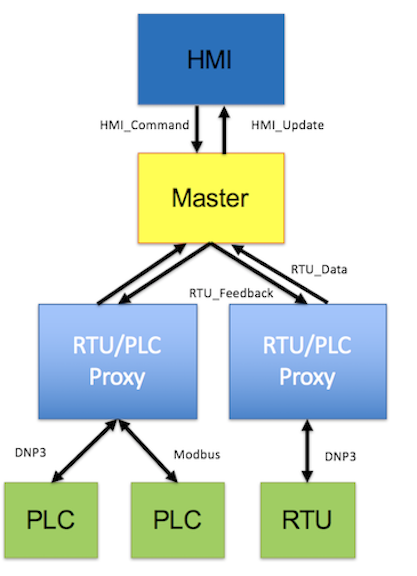
\includegraphics{new_architecture}
  \caption{Event-Based Architecture}
  \label{fig:2}
  \end{center}
\end{figure}

\indent \indent
The architecture of the system is presented in figure \ref{fig:2}. The arrows describe
the direction of message flow, with the labels being the type of messages. The system
supports any configuration of PLC/RTU Proxies as well as PLCs and RTUs
with PLC/RTU Proxies able to support multiple
PLCs of different protocol communication types. 
This configuration is described in a json config file. 
Information such as the IP address of the PLCs, the communication protocols they use,
the registers to poll (if Modbus), which PLC's correspond to which PLC/RTU Proxy,
and the ports all the PLCs listening on are all described in this configuration file. 
The system currently supports DNP3 and Modbus, but it is extendable to allow
easy extension to future protocols. The cJSON library is used to parse
the JSON \cite{cJSON}.\\

\indent
The packet types \code{HMI\_Command}, \code{HMI\_Update}, \code{RTU\_Feedback},
and \code{RTU\_Data} are used to route different types of messages
around the system.
The PLC Proxy gets data from it's PLCs or RTUs speaking either Modbus or DNP3,
and sends this up to the
SCADA Master in a \code{RTU\_Data} message whenever there is a change of state.
This message is not in any SCADA
protocol, but contains bundled information about the PLCs that the master
needs in a IP packet. The SCADA Master processes this message, updates it's state, and then sends the
HMI a \code{HMI\_Command} message that has all the information the HMI needs
to visualize the scenario. The HMI processes this message to present the viewer with
the monitoring information. If the monitor clicks a button, the HMI 
recognizes this event and sends an \code{HMI\_Command} message to the SCADA Master.
The SCADA Master receives this command, uses the information in the configuration 
file to determine what proxy to forward
this message to, and sends a \code{RTU\_Feedback} message to that proxy. 
That proxy then uses
the configuration information to determine which PLC to route this message to, and translates
the feedback message into a command message in the given PLC's communication
protocol. \\

\indent    
The code for this project is released as a part of the Spire 1.0. All of the
file names I will use to describe where code is located are the file names
used in the Spire 1.0 release. The config file previously mentioned is located
in \code{config/config.json}, and the packet definitions are located in
\code{common/scada\_packets.h}. \\


\section{pvbrowser HMI}

\begin{figure}[ht]
  \begin{center}
  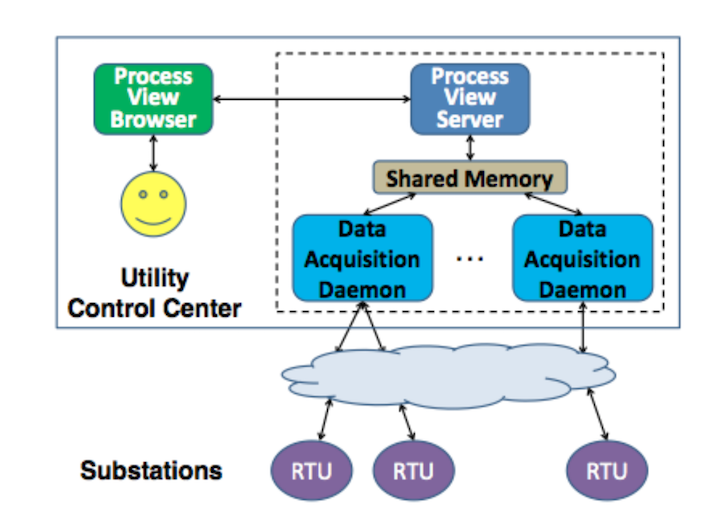
\includegraphics{pvb_architecture}
  \caption{pvbrowser Stock Architecture \cite{towardsscada}}
  \label{fig:3}
  \end{center}
\end{figure}

\indent \indent
We base our HMI on pvbrowser \cite{pvbrowser}.
pvbrowser is an open-source SCADA 
software suite. It has been used to manage a real SCADA system deployment
in Romania spanning 10,000 square kilometers with 50 power switches \cite{pvbrowser}.
It is a full SCADA solution - it provides an HMI and a SCADA Master with Modbus
data acquisition daemons that can communicate with RTUs. It's architecture is pictured
in \ref{fig:3}. Early work made it clear that replicating pvbrowser has some of the
same difficulties Kirsch et al. described in \cite{SurvivableSCADA}
, but the software includes several useful components, such as the HMI and Modbus
communication. 
We rearchitected the HMI to remove the shared memory and
data acquisition daemons, and replaced them with a thread that communicates with our
SCADA Master and supplies the pvbrowser thread with the most up to date information of
how to visualize the system. When there is a button click, the pvbrowser thread
sends a message to the SCADA master. \\

\indent 
This code is located in the \code{hmi} folder. \code{hmi/master\_exec.cpp} contains the thread
that reads from the SCADA master and update's the pvbrowser data structures.
\code{hmi/mask1\_slots.h} contains the code both to visualize the HMI based on the
current data structures, as well as the code to send \code{HMI\_Command} messages
when buttons are clicked. \\

\section{SCADA Master}

\indent \indent


The SCADA Master maintains the global view of the system. It has all the monitoring
data from the PLC/RTU proxy, and sends the HMI all the data it needs to monitor.
It is also the program that forwards operator commands from the HMI to the proxies.
The SCADA master server runs a switch
statement waiting for different message types. When it receives an \code{HMI\_Command}
message, it calls the \code{read\_from\_hmi} method which discovers what the corresponding
\code{RTU\_Feedback} message
should be doing (what field of a RTU it will be modifying) and where to route it (using the config
file),
and then sends it to the proxy. When it receives an \code{RTU\_Data} message, it updates
it's data structures, then calls the \code{process} method. This method is unique
to each individual scenario. After processing the latest update from the HMI it 
will craft an \code{HMI\_Update} message
and send it to the HMI. \\

\indent
The SCADA master is built from scratch in C. It is located in \code{master/scada\_master.c}
and it's data structures are in \code{master/structs.h}. \\

\section{PLC/RTU Proxy}
\begin{figure}[ht]
  \begin{center}
  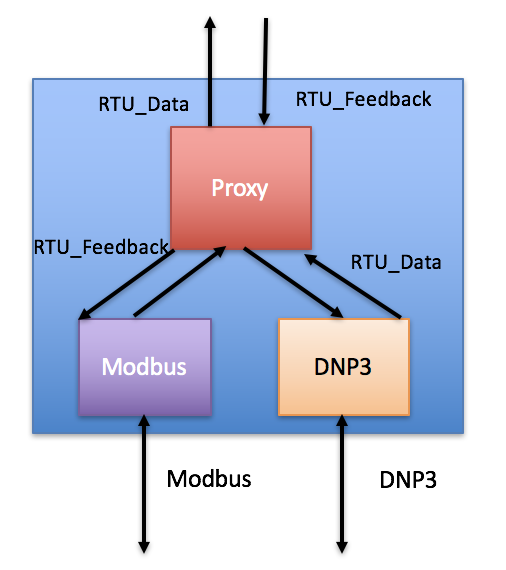
\includegraphics{proxy}
  \caption{PLC/RTU Proxy Architecture}
  \label{fig:4}
  \end{center}
\end{figure}

\indent \indent
The PLC/RTU Proxy communicates with PLC's directly, forwarding their updates
to the SCADA Master and forwarding command messages from the SCADA Master to the specific
PLC.
The architecture of the PLC/RTU Proxy is shown in figure \ref{fig:4}. The Proxy
process is located in \code{proxy/proxy.c}. When it runs, it checks it's configuration
to determine PLCs or RTUs it is responsible for, and what processes they run.
If there are any PLCs that speak Modbus, it spawns the process 
\code{modbus/modbus\_master}. If it is responsible for any PLCs that speak DNP3 it spawns
the process \code{dnp3/dnp3\_master}. It is set up that if there are any more protocols
implemented, it would spawn their daemon as well. The daemon processes are designed
such that they can handle multiple PLCs of the same protocol. For example, if the
proxy is responsible for three PLCs that speak Modbus, it will only spawn one Modbus
 daemon process. A IPC channel is created for each of the 
child data acquisition daemons such that the proxy can communicate to the child and the
child can communicate with the proxy. When the proxy gets an \code{RTU\_Feedback} message,
it checks to see what protocol the destination PLC speaks and forwards the 
\code{RTU\_Feedback} message to the designated daemon. 
When the proxy receives \code{RTU\_Data}
messages from its children, the proxy forwards those messages to the SCADA master. \\

\indent
The Modbus daemon is based on pvbrowser's Modbus data acquisition daemon
from pvbaddons \cite{pvbrowser}.
The code is located at \code{modbus/modbus\_master.cpp}. 
It reads the configuration file to determine the PLCs that it needs to connect with.
It then creates TCP connections with them and starts
the Modbus polling protocol. Every time out it polls the PLCs at the location
specified in the config file, and then forwards an \code{RTU\_Data} message with
the corresponding information to the proxy over IPC. If the Modbus daemon recieves
an \code{RTU\_Feedback} message, it will translate this into the proper Modbus
control message and forward this to the corresponding PLC. \\

\indent
The DNP3 daemon process uses the OpenDNP3 library (\cite{OpenDNP3}) to implement 
DNP3 communication with it's devices. DNP3 is a more advanced event-based communication
protocol that is common in power grid networks. OpenDNP3 provides a modern, C++11 
programming API for implementing DNP3 communication. We have even contributed
to the OpenDNP3 project through a bug fix. The code for the DNP3 daemon is in
\code{dnp3/}. The file \code{dnp3/main.cpp} is responsible for reading the configuration file
to determine what PLCs it has to communicate with, and starting a DNP3 session with 
those PLCs. It sets up callback functions for these PLCs, such that when they send an event
update, the code in \code{dnp3/callback.cpp} runs, and creates an \code{RTU\_Data}
message to be sent to the proxy process. The main thread also sets up IPC communication
with the proxy such that when it gets an \code{RTU\_Feedback} message it translates
this into a DNP3 control message and sends it along to the corresponding PLC. \\


\section{OpenPLC}

\indent \indent 
We use OpenPLC \cite{OpenPLC} to emulate PLCs and RTUs. It is very useful, as
it allows us to emulate realistic PLCs that a SCADA system would have to
control and monitor. In addition to emulation, the OpenPLC software can be deployed to 
many hardware platforms to create a physical PLC. \\

\indent 
OpenPLC is configured by creating a Ladder Logic (LD) or Structured Text (ST) 
description of the PLC. Variables
can be mapped to register positions on the PLC, and manipulated with the
Ladder Logic or Structured Text. These same registers map to Modbus registers. Devices
can then communicate with the OpenPLC via Modbus by polling for the desired registers. \\

\indent
We extended OpenPLC to also map the registers to DNP3 addresses and communicate with 
masters via DNP3. This is done with OpenDNP3, and allows us to emulate a wider variety
of devices. Now, when OpenPLC runs, it listens for both Modbus or DNP3 communication,
and can actually communicate with both at the same time.

\chapter{Case Study: Power Distribution Scenario}

\section{Overview}

\indent \indent
To demonstrate our system in a realistic SCADA environment we built a power distribution
case study. The case study is designed with ten PLCs providing the system with power switching
information according to the topology in Figure \ref{fig:5}. An operator can monitor and control
this emulated topoploy, and use it to route power around different
substations. The scenario models what a real operator would see, it is modeled after
the Lucy Electric Scada System \cite{lucy}. \\

\indent
In the scenario, power is in the
primary substation. All of the auxiliary  substations (Port, Johns Hopkins,
Rural Community, The Metropolitan Area) need to be powered. For substations
to distribute power, their transformers must be on. For power lines to cary
power, the switches at both ends must be closed.There are spare
links in operation if power lines go down. Their switches at both ends are open,
so power can't flow. If a power line goes down, both the switches at both ends
will trip.  The operator will see this, and react by using the lines that aren't
in use to route power to the substations that now do not have it. \\

\section{HMI}
\begin{figure}[ht]
  \begin{center}
  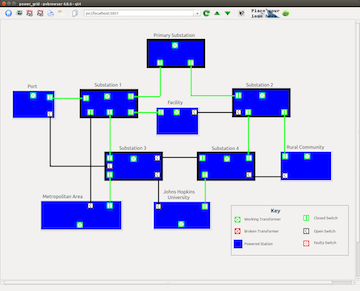
\includegraphics{normal_operation}
  \caption{A pvbrowser-based HMI}
  \label{fig:5}
  \end{center}
\end{figure}

\indent \indent
The HMI is presented in Figure \ref{fig:5}. The boxes are substations - if they are
blue there is power located at the substation.  If a substation is black then that
substation has no power. The 'X' in the middle of a substation is a transformer. 
If it is red, then it is off. If it is green, it is on.
If switches are green
they are closed, if they are black they are open, and if they are red they are tripped.
 When switches
are open or tripped, power cannot flow through a line and thus it is black. When switches
are both closed, and one of the substations has power, then power will flow
through the line and it will be green. \\

\indent
An operator can change the state of the system by pointing and clicking. If the operator
clicks a transformer, that transformer will turn on or off (whichever is the opposite
of it's current state). When an operator
clicks on a switch, that switch will close if it is open or open if it is closed. An
operator cannot effect the status of a tripped switch because it requires maintenance
by a crew in the real world. An example of the HMI when a switch is tripped and there
is a blackout is in Figure \ref{fig:13}.


\begin{figure}[ht]
  \begin{center}
  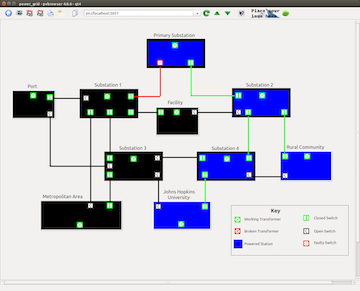
\includegraphics{dead_link_screen_shot}
  \caption{The HMI When A Power Link Dies}
  \label{fig:13}
  \end{center}
\end{figure}


\section{SCADA Master}

\indent \indent

The SCADA master for this scenario runs a version of breadth first search to determine
what substations are powered, and what lines are carrying electricity. It does this because
it knows from the PLCs only which switches are open or closed, and which transformers are
on or off. Only the primary substation is known to be powered, and the rest of the 
information for the operator has to be extrapolated from the data the PLCs are providing.
It takes the result of this process and sends it to the HMI in a 
\code{HMI\_Update} message.
\\

\indent
The master is able to translate \code{HMI\_Command} messages, which come from the HMI and 
specify what item has been pressed, into \code{RTU\_Feedback} messages, that are tagged to 
a specific PLC and Proxy, and, if the item pressed is a switch, contain the specific
register number the switch should correspond to. \\

\section{RTU/PLC Proxy}

\indent \indent
In this system setup there is a proxy for each PLC, so a total of 10 proxies are run.
This is because each PLC is supposed to be located at a different location. \\

\indent
The proxies protocol daemons know how to translate a \code{RTU\_Feedback} message
into a corresponding Modbus or DNP3 message to send to the PLC or RTU. For DNP3,
switch controls are Analog Output Commands and the transformers are CROB 
instructions. For Modbus, the switch controls send a set register command and
the transformers are force coil commands. These are different types of commands
used to modify different types of  registers.

\section{PLC Emulation}

\begin{figure}[ht]
  \begin{center}
  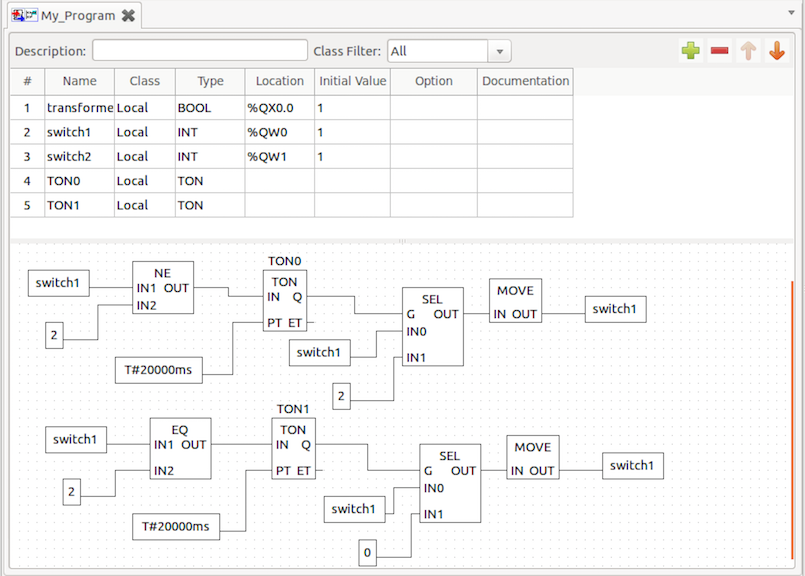
\includegraphics{open_plc}
  \caption{Ladder Logic for RTU 0 in OpenPLC}
  \label{fig:6}
  \end{center}
\end{figure}

\indent \indent
To run this scenario we emulated 10 PLCs - one for each substation. The first
three PLCs are emulated with OpenPLC using DNP3. The next two PLCs are emulated with
OpenPLC using Modbus. To demonstrate our system's backwards compatibility, we also emulate
five PLCs with the ASE Test Set 2000 Device \cite{ASE}. It can emulate
Modbus or DNP3 RTUs. The next three
PLCs are emulated with the ASE device through DNP3, and the last two are emulated
with the ASE device through Modbus. \\

\indent
The PLCs contain data for the transformers and switches. A switch value of 0 is open,
1 is closed, and 2 is tripped. A transformer value of 1 is on and 0 is off.
This data is represented in
two different ways depending on if the device is Modbus or DNP3. If the device is 
Modbus, the transformer is a coil status at register zero, and the switches are 
holding registers at the register it's switch number should be (if a substation
has three switches it will have holding registers at 0, 1, 2 to store that switch's 
data). For DNP3, the registers for the transformers and switches are at the same location
, but instead of Coil Status and Holding Registers it is Binary Output Status
and Analog Output Status. \\

\indent
In this scenario, PLC 0 (the primary substation) has been written with Ladder Logic
in OpenPLC. The associated LD program is shown in figure \ref{fig:6}. This program
trips the first switch every 20 seconds, and then un-trips it and sets the status
to open every other 20 seconds. \\

\chapter{Conclusion}

\indent \indent
We have introduced an open-source event-based architecture for SCADA systems.
This new architecture allows for easier replication of the SCADA master, is more
scalable than many current SCADA architectures, is more secure with
the PLC / RTU Proxy component, and should have an easier path to adoption thanks
to being open-source and backward compatibility with devices. 
This architecture is used by the Spire Intrusion-Tolerant SCADA System for the Power Grid \cite{Spire}.\\

\appendix


\bibliographystyle{unsrt}
\bibliography{sample}

\end{document}

